% AY = r
\begin{center}
    \textcrimson{\textbf{\Huge AY = r}}\\
    \textbf{\large Solution by Azzam L. H.}
\end{center}

\section{Soal}
Diberikan segitiga $ABC$ dengan $AB \neq AC$. Misalkan titik $I$ adalah pusat lingkaran dalam dan $r$ adalah panjang jari-jari lingkaran dalam segitiga $ABC$. Definisikan $X$ sebagai titik tengah $BC$ dan $Y$ sebagai perpotongan $XI$ dengan garis tinggi dari $A$. Buktikan bahwa panjang $AY = r$.

\begin{center}
\definecolor{wewdxt}{rgb}{0.43137254901960786,0.42745098039215684,0.45098039215686275}
\definecolor{rvwvcq}{rgb}{0.08235294117647059,0.396078431372549,0.7529411764705882}
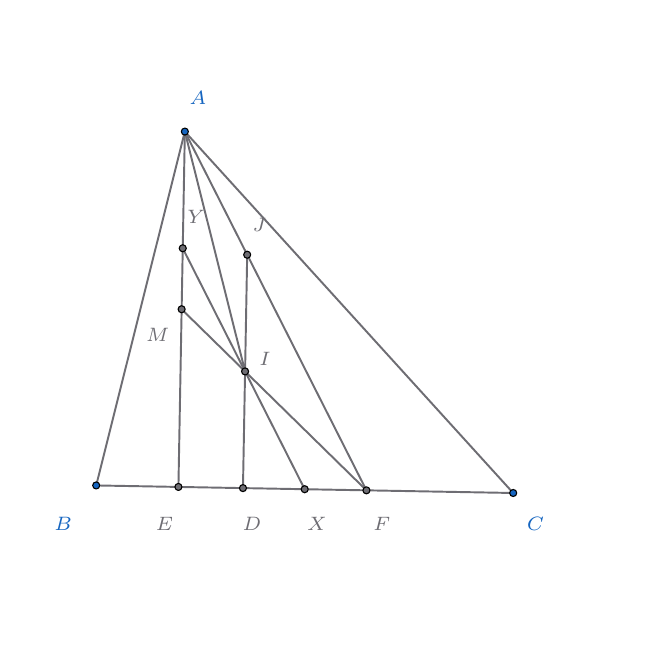
\begin{tikzpicture}[line cap=round,line join=round,scale=1.5]
\clip(-2,-4) rectangle (3,1);
\draw [line width=0.7pt,color=wewdxt] (-0.6691878889233828,0.12035559271907031)-- (-1.4198185816696804,-2.8757554817472792);
\draw [line width=0.7pt,color=wewdxt] (-1.4198185816696804,-2.8757554817472792)-- (2.1108121110766174,-2.93964440728093);
\draw [line width=0.7pt,color=wewdxt] (2.1108121110766174,-2.93964440728093)-- (-0.6691878889233828,0.12035559271907031);
\draw [line width=0.7pt,color=wewdxt] (-0.6964101052115195,-1.3839989029728486)-- (-0.1593091626400931,-1.9103101410210563);
\draw [line width=0.7pt,color=wewdxt] (0.8681799183974734,-2.9171582164179477)-- (-0.1593091626400931,-1.9103101410210563);
\draw [line width=0.7pt,color=wewdxt] (-0.6691878889233828,0.12035559271907031)-- (-0.1593091626400931,-1.9103101410210563);
\draw [line width=0.7pt,color=wewdxt] (-0.1593091626400931,-1.9103101410210563)-- (-0.1771863889905364,-2.8982416726102604);
\draw [line width=0.7pt,color=wewdxt] (-0.6870651152738262,-0.8675759388701335)-- (0.34549676470346846,-2.9076999445141043);
\draw [line width=0.7pt,color=wewdxt] (-0.7236323214996562,-2.8883533986647674)-- (-0.6691878889233828,0.12035559271907031);
\draw [line width=0.7pt,color=wewdxt] (0.8681799183974734,-2.9171582164179477)-- (-0.6691878889233828,0.12035559271907031);
\draw [line width=0.7pt,color=wewdxt] (-0.14143193628964976,-0.922378609431852)-- (-0.1593091626400931,-1.9103101410210563);
\begin{scriptsize}
\draw [fill=rvwvcq] (-0.6691878889233828,0.12035559271907031) circle (0.85pt);
\draw[color=rvwvcq] (-0.5574181086923242,0.40469108281135935) node {$A$};
\draw [fill=rvwvcq] (-1.4198185816696804,-2.8757554817472792) circle (0.85pt);
\draw[color=rvwvcq] (-1.7,-3.2) node {$B$};
\draw [fill=rvwvcq] (2.1108121110766174,-2.93964440728093) circle (0.85pt);
\draw[color=rvwvcq] (2.3,-3.2) node {$C$};
\draw [fill=wewdxt] (0.34549676470346846,-2.9076999445141043) circle (0.85pt);
\draw[color=wewdxt] (0.45,-3.2) node {$X$};
\draw [fill=wewdxt] (-0.7236323214996562,-2.8883533986647674) circle (0.85pt);
\draw[color=wewdxt] (-0.8409797974464288,-3.2) node {$E$};
\draw [fill=wewdxt] (-0.6964101052115195,-1.3839989029728486) circle (0.85pt);
\draw[color=wewdxt] (-0.9,-1.6) node {$M$};
\draw [fill=wewdxt] (-0.1593091626400931,-1.9103101410210563) circle (0.85pt);
\draw[color=wewdxt] (0.009705268815885258,-1.8) node {$I$};
\draw [fill=wewdxt] (-0.1771863889905364,-2.8982416726102604) circle (0.85pt);
\draw[color=wewdxt] (-0.1,-3.2) node {$D$};
\draw [fill=wewdxt] (0.8681799183974734,-2.9171582164179477) circle (0.85pt);
\draw[color=wewdxt] (1,-3.2) node {$F$};
\draw [fill=wewdxt] (-0.6870651152738262,-0.8675759388701335) circle (0.85pt);
\draw[color=wewdxt] (-0.57317153584533,-0.6035282549810136) node {$Y$};
\draw [fill=wewdxt] (-0.14143193628964976,-0.922378609431852) circle (0.85pt);
\draw[color=wewdxt] (-0.037555012643132185,-0.6665419635930369) node {$J$};
\end{scriptsize}
\end{tikzpicture}
\end{center}

\newpage
\section{Solusi}

\begin{proof}[\textbf{Solusi. }]
    The well known lemma mentioned here are already proven here: \\
    \url{https://artofproblemsolving.com/community/c473124h1565787_diameter_of_incircle_and_midpoints_of_altitudes}

\begin{center}
\definecolor{wewdxt}{rgb}{0.43137254901960786,0.42745098039215684,0.45098039215686275}
\definecolor{rvwvcq}{rgb}{0.08235294117647059,0.396078431372549,0.7529411764705882}
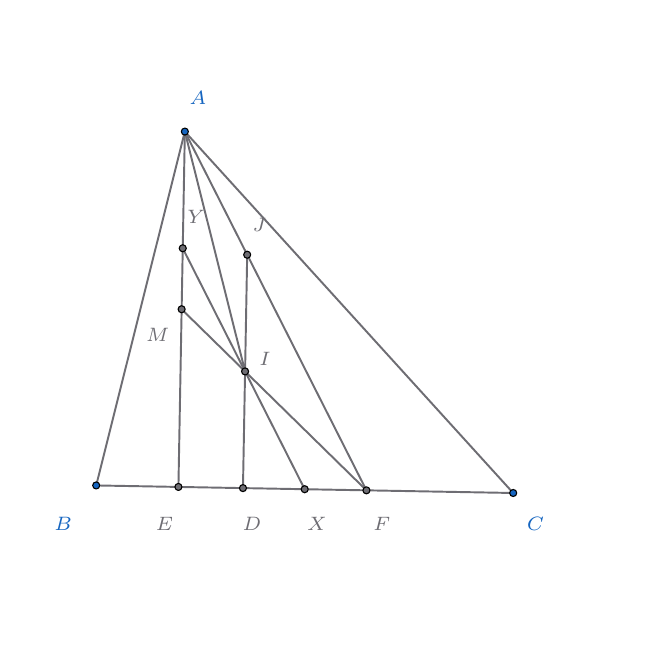
\begin{tikzpicture}[line cap=round,line join=round,scale=1.5]
\clip(-2,-4) rectangle (3,1);
\draw [line width=0.7pt,color=wewdxt] (-0.6691878889233828,0.12035559271907031)-- (-1.4198185816696804,-2.8757554817472792);
\draw [line width=0.7pt,color=wewdxt] (-1.4198185816696804,-2.8757554817472792)-- (2.1108121110766174,-2.93964440728093);
\draw [line width=0.7pt,color=wewdxt] (2.1108121110766174,-2.93964440728093)-- (-0.6691878889233828,0.12035559271907031);
\draw [line width=0.7pt,color=wewdxt] (-0.6964101052115195,-1.3839989029728486)-- (-0.1593091626400931,-1.9103101410210563);
\draw [line width=0.7pt,color=wewdxt] (0.8681799183974734,-2.9171582164179477)-- (-0.1593091626400931,-1.9103101410210563);
\draw [line width=0.7pt,color=wewdxt] (-0.6691878889233828,0.12035559271907031)-- (-0.1593091626400931,-1.9103101410210563);
\draw [line width=0.7pt,color=wewdxt] (-0.1593091626400931,-1.9103101410210563)-- (-0.1771863889905364,-2.8982416726102604);
\draw [line width=0.7pt,color=wewdxt] (-0.6870651152738262,-0.8675759388701335)-- (0.34549676470346846,-2.9076999445141043);
\draw [line width=0.7pt,color=wewdxt] (-0.7236323214996562,-2.8883533986647674)-- (-0.6691878889233828,0.12035559271907031);
\draw [line width=0.7pt,color=wewdxt] (0.8681799183974734,-2.9171582164179477)-- (-0.6691878889233828,0.12035559271907031);
\draw [line width=0.7pt,color=wewdxt] (-0.14143193628964976,-0.922378609431852)-- (-0.1593091626400931,-1.9103101410210563);
\begin{scriptsize}
\draw [fill=rvwvcq] (-0.6691878889233828,0.12035559271907031) circle (0.85pt);
\draw[color=rvwvcq] (-0.5574181086923242,0.40469108281135935) node {$A$};
\draw [fill=rvwvcq] (-1.4198185816696804,-2.8757554817472792) circle (0.85pt);
\draw[color=rvwvcq] (-1.7,-3.2) node {$B$};
\draw [fill=rvwvcq] (2.1108121110766174,-2.93964440728093) circle (0.85pt);
\draw[color=rvwvcq] (2.3,-3.2) node {$C$};
\draw [fill=wewdxt] (0.34549676470346846,-2.9076999445141043) circle (0.85pt);
\draw[color=wewdxt] (0.45,-3.2) node {$X$};
\draw [fill=wewdxt] (-0.7236323214996562,-2.8883533986647674) circle (0.85pt);
\draw[color=wewdxt] (-0.8409797974464288,-3.2) node {$E$};
\draw [fill=wewdxt] (-0.6964101052115195,-1.3839989029728486) circle (0.85pt);
\draw[color=wewdxt] (-0.9,-1.6) node {$M$};
\draw [fill=wewdxt] (-0.1593091626400931,-1.9103101410210563) circle (0.85pt);
\draw[color=wewdxt] (0.009705268815885258,-1.8) node {$I$};
\draw [fill=wewdxt] (-0.1771863889905364,-2.8982416726102604) circle (0.85pt);
\draw[color=wewdxt] (-0.1,-3.2) node {$D$};
\draw [fill=wewdxt] (0.8681799183974734,-2.9171582164179477) circle (0.85pt);
\draw[color=wewdxt] (1,-3.2) node {$F$};
\draw [fill=wewdxt] (-0.6870651152738262,-0.8675759388701335) circle (0.85pt);
\draw[color=wewdxt] (-0.57317153584533,-0.6035282549810136) node {$Y$};
\draw [fill=wewdxt] (-0.14143193628964976,-0.922378609431852) circle (0.85pt);
\draw[color=wewdxt] (-0.037555012643132185,-0.6665419635930369) node {$J$};
\end{scriptsize}
\end{tikzpicture}
\end{center}






    Misalkan $E$, $D$, $F$, $M$, dan $J$ berturut-turut adalah kaki tinggi dari $A$ ke $BC$, titik singgung lingkaran dalam $ABC$ dengan $BC$, refleksi $D$ terhadap $X$, titik tengah $AE$, dan refleksi $D$ terhadap $I$.

    Perhatikan dari beberapa lemma yang cukup terkenal, kita punya $A,J,F$ segaris, dan $M,I,F$ segaris.

    Karena $DI = IJ$ dan $DX = XF$ berarti $XI \parallel FJ$. Karena $AY \perp BC$ dan $JI \perp BC$ maka didapat juga $AY \parallel JI$. Dari dua fakta tersebut dapat disimpulkan bahwa $AJIY$ jajar genjang sehingga $AY = JI = r$. Terbukti.
\end{proof}
